\section{Product perspective}
\label{sec:product_perspective}%

\subsection{Scenarios}
\label{subsec:scenarios}%
\paragraph{Scenario 1: Unregistered ST creates an account}
Aldo Pinesco is looking for an internship to get a taste of the working world, so he decides to join S\&C. First, he opens the website and clicks on the Sign-up button, then he inserts his name, surname, email and password in order to create a new account.

\paragraph{Scenario 2: ST updated their resume}
When the student Cristiano Prendano has created his account on S\&C platform, for make his profile visible to the CPs, he must to upload his CV. 
When Cristiano tries to upload his CV the S\&C asks him to answer questions about CV such as his skills, attitudes and interests.

\paragraph{Scenario 3: CP creates and publishes a new internship}
The Lazzari Company, which is an established company in the Cybersecurity field, wants to offer a professional internship and reach out to as many students as possible. For doing so, they use the S\&C system, so they first define the internship domain by choosing from the several available options, then they define the topics and technologies adopted still using the suggestions offered by the system, and finally they also define the terms of the internship, such as the possibility of being paid or other benefits that a company can offer. Finally, by clicking on the "Publish" button, the internship will be added to the company's showcase, which can be seen from everyone, and also to the system's database, on which the recommendation algorithm works, so that it can immediately start working to find potentially suitable people.

\paragraph{Scenario 4: CP updates or removes an internship}
One month ago, Corean Company published an internship for four students. During the last month 3 student have been accepted, so the Corean Company logs in their account, open his posts section, search for the internship and update the available position.

\paragraph{Scenario 5: ST receives internship recommendations}
The student Riccardo Pianabasso, who has already uploaded his information, has received a notification from the system informing him about a new internship match. After clicking on the message inbox section, he finds a message with all the information about the internship to which he has been matched. Now he has two options, accept or reject the internship. If he refuses, the match is discarded from the system and the company is notified; if he accepts the system will show either that the company has already accepted/rejected the student for the interview or that the company response is pending.

\paragraph{Scenario 6: ST apply for an internship}
After finding an internship suitable for him, the student Mirco Opaco , click on the apply button and waits for the company response.
The system sends to company the application request by Mirco Opaco that will be reviewed.

\paragraph{Scenario 7: CP reviews applications for an internship}
The fintech company Sossoldi is looking for an intern to join their budget management team. Their ad received several applications via S\&C. Marco Lazzaro, the hiring manager, accesses the "Applications" section, where he reviews the details of each candidate. After going through their CVs and motivational letters, he selects the three best candidates and contacts them.

\paragraph{Scenario 8: CP contacts a student for an internship}
After finding a suitable student for the Company, the hiring manager opens the student profile and sends an application request to the student for an internship.
The system sends a notification to the student about the application request.

\paragraph{Scenario 9: CP conducts interviews for candidates}
After both parties accept the application, the company begins to construct questionnaires or tasks to be submitted to the applicant, using the help provided by the system. Once this phase is completed, the company sends the material to the students, who can start the assignments. The system then collects the information and sends it to the company, which can decide how to proceed based on its own policies, such as requiring a personal interview, completing other tasks, or accepting the student.

\paragraph{Scenario 10: User makes a complaint}
While working at Pizza Tech, Emily realizes that her task are different from what was written in the internship description. So she logs into the S\&C platform, goes to the internship page and clicks on the button "File a complaint". Emily fills out the form, clearly stating the differences between the job description and the actual tasks assigned. The complaint is automatically forwarded to her university.

\paragraph{Scenario 11: Users provide feedback after an internship}
After completing his internship at BioTech, Lorenzo receives a notification from S\&C asking him to leave feedback about his experience. He fills out a form indicating aspects such as the skills he gained, the support received from the company, and the clarity of objectives. At the same time, his mentor at BioTech fills out a similar form to evaluate Lorenzo, highlighting his problem-solving skills and enthusiasm. Both feedbacks are stored in the system and will be used to improve future matches.

\paragraph{Scenario 12: UV monitors internship progress}
The responsible for students participating in the internships periodically logs in in the S\&C system and monitors the progress of students at his university through the list the systems shows him on his home page.

\paragraph{Scenario 13: UV handles complaints}
The university receives a notification from S\&C about a complaint about one of its students. A partner company has reported that a student failed to show up for a scheduled interview. The university reviews the case details, contacts the student for clarification and sends a response to the company with an explanation and an approach to avoid similar issues in the future.

\paragraph{Scenario 14: S\&C notifies Users about a new matching}
Every day, the S\&C system runs its recommendation algorithms to identify matches between students and internships based on their profiles, preferences, and internship criteria. For instance, Chiara Lombardi, a computer science student specializing in artificial intelligence, receives a notification from S\&C about a new internship opportunity at NeuralNet Solutions. The system highlights that this internship involves working on a project with AI-based recommendation systems, which aligns with Chiara's skills and preferences.

Chiara logs into her account, opens the "Notifications" section, and clicks on the recommended internship. She reviews the details and decides whether to express her interest in the position or dismiss the recommendation. Similarly, NeuralNet Solutions is notified about Chiara's profile matching their internship requirements. They can review her CV and decide whether to contact her for further evaluation.

\paragraph{Scenario 15: S\&C updates ST on the progress of their application}
Franco applied for a data science internship offered by HugeData through the S\&C system. A few days later, he receives a notification that his application has been accepted and he is scheduled for an interview. In the notification, he finds the interview details: the date, time, and a link to join. He confirms his availability by clicking "Accept interview".

\subsection{Class diagrams}
\label{subsec:class_diagrams}%

\begin{figure}[H]
    \begin{center}
        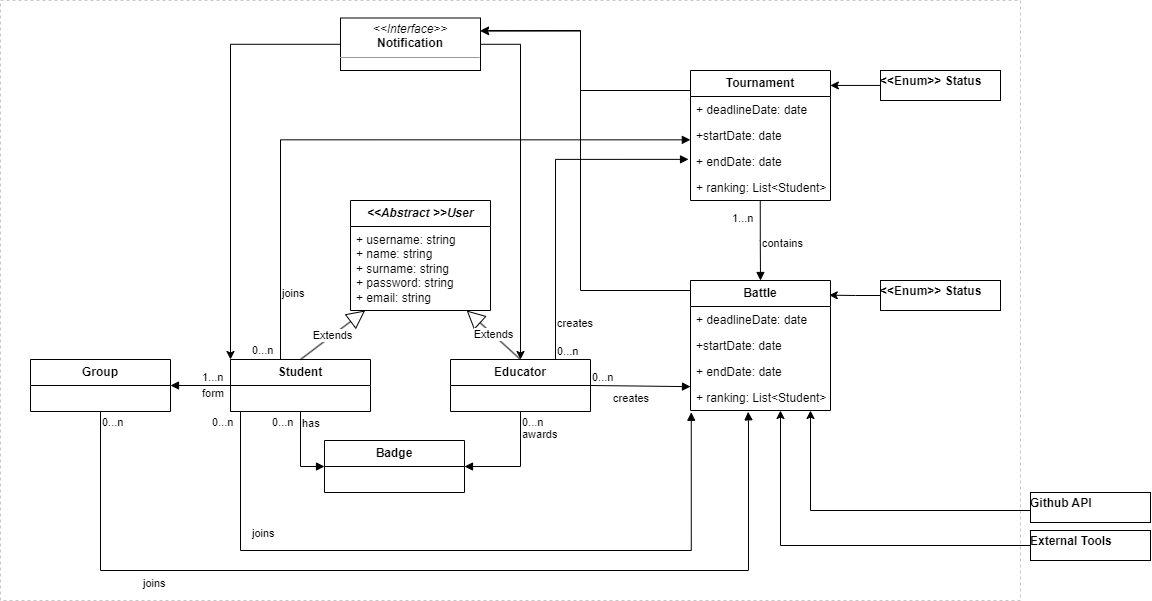
\includegraphics[width=0.9\linewidth]{UML.png}
        \caption{High level Class Diagram.}
        \label{fig:UML}%
    \end{center}
\end{figure}

The UML class diagram illustrates the key entities and their relationships within the system. The Student entity represents users seeking internships, with attributes such as studentId, name, email, and resume. Students can apply for internships and are matched with recommendations generated by the system. The Company manages multiple internships and receives recommendations, which are lists of students matching their criteria.

The Recommendation entity, generated by internships and students, connects students to opportunities based on their profiles and scores. Notifications, represented by the Notification interface, are sent to both students and companies, informing them of recommendations updates. The University oversees internships by monitoring their progress and handling Complaints, submitted by students or companies, which include attributes like description and status.

Lastly, Feedback, provided by students and companies, helps improve the internship experience. Relationships such as publishes, monitors, handles, and provides ensure clear responsibilities and interactions between entities, supporting a robust and scalable system.\\


\subsection{State diagrams}
\label{subsec:state_diagrams}%
In this section are presented the State Diagrams of the S\&C system representing possible operations that a user can perform.
TODO

\paragraph{Name}
Brief description

\begin{figure}[H]
    \begin{center}
        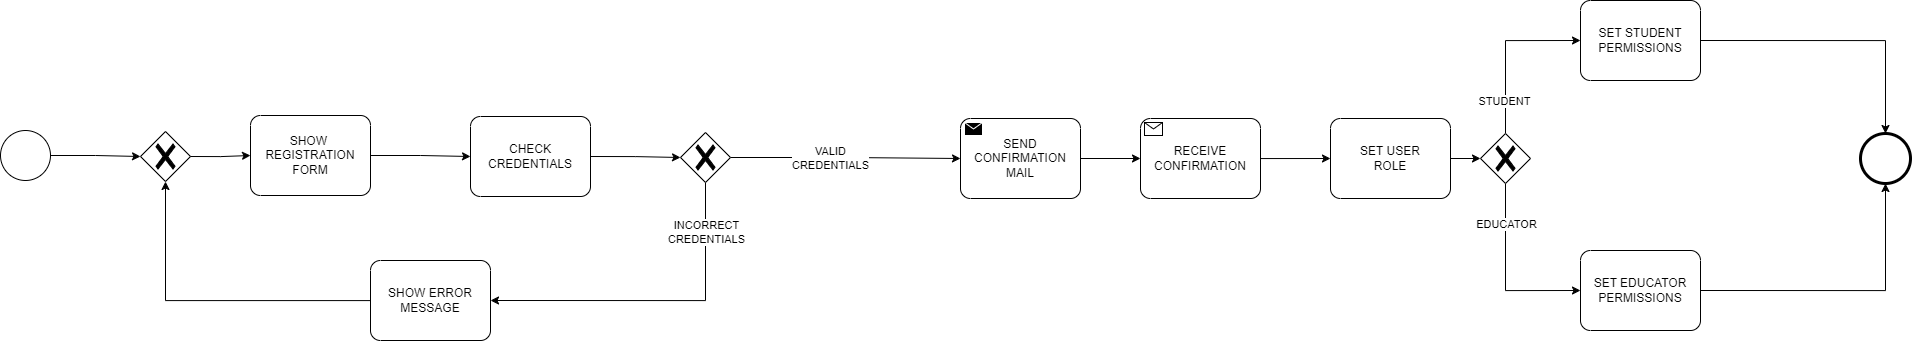
\includegraphics[width=1\linewidth]{StateDiagrams/signup.png}
        \caption{Figure}
        \label{fig:signup_sd}%
    \end{center}
\end{figure}

Repeat

\section{Product functions}
\label{sec:product_functions}%
Here are listed a summary of the main functions of the S\&C system:\\\\
\textbf{ Sign-up:} The User submits his name, surname, email address and a new password. A confirmation mail is required to complete the process.\\\\
\textbf{ Login:} The User sign in after typing his email and password in the login form. \\\\  
\textbf{ Update CV:} A ST can update their data after creating a new account, including experience, skills, attitude and the resume .\\\\
\textbf{ Publish an internship:} A CP can publish an internship proposal through  the "create new internship" section.\\\\
\textbf{ Search for an internship:} A ST can look for an internship by keyword search or by setting some predefined filters, even both simultaneously.\\\\
\textbf{ Apply for an internship:} A ST can apply for an internship by clicking on the "Apply" button on an internship post.\\\\
\textbf{ Ask for a ST application: } A CP can send a notification of interest to a student from the list of recommendations provided by the system.\\\\
\textbf{ Reviewing an apply request:} A company can decide whether to accept or reject a student's application from the application section or after receiving a notification via the inbox.\\\\
\textbf{ Create task for interviews:}  A CP can prepare tasks or questionnaires to evaluate candidates through the system's interview management section. These tasks may include technical challenges, situational assessments, or other relevant exercises, which are assigned to candidates. Once the tasks are completed and reviewed, the CP can schedule further interviews directly through the system, specifying the date, time, and format, and notifying candidates. \\\\
\textbf{ Solve tasks and questionnaires:} A ST can access and complete the tasks or questionnaires assigned by a CP through their profile. After submission, the system automatically records their responses and notifies the CP about the completion, allowing them to evaluate the candidate's performance.\\\\
\textbf{ Finalize selections :} After reviewing completed tasks and conducting interviews, a CP can finalize their selections for an internship position. This includes marking the selected students and notifying them through the system, while also sending updates to unselected candidates.
\\\\
\textbf{ Logout:} A User session will be closed if the User clicks on "Logout" button. Next time the User opens S\&C he will need to log in again.

\section{User characteristic}
\label{sec:User_characteristic}%
There are three types of users in the S\&C platform: Students (STs), Companies (CPs) and Universities (UVs). Below is a description of their main characteristics and functionalities within the platform.
\begin{itemize}
    \item ST: Students are users seeking internships to gain experience or fulfill academic requirements. They can register and log in to the platform by providing their personal details, educational background, and resume. Once registered, they can:
    \begin{itemize}
        \item Search for available internships.
        \item Apply for internships that match their interests.
        \item Receive personalized internship recommendations based on their profiles.
        \item Accept or reject internship offers.
        \item Provide feedback on their internship experiences after completing them.
    \end{itemize}
    \item CP: Companies use the platform to find suitable candidates for their internships and ease the selection process. Companies must provide basic information about their organization when registering and then they can:
    \begin{itemize}
        \item Create, publish, update, or remove internship postings.
        \item Search for students who match their requirements.
        \item Review applications and contact students.
        \item Conduct interviews and finalize candidate selection.
        \item Provide feedback about students post-internship.
    \end{itemize}
    \item UV: Universities act as a supervisor to ensure proper conduct of internships. Universities have access to the feedback and status of internships to maintain oversight and address issues effectively. Universities must provide basic information about them when registering and their primary responsibilities are:
    \begin{itemize}
        \item Monitoring the progress of internships.
        \item Handling complaints or disputes raised by students or companies.
        \item Ensuring compliance with academic and professional standards.
    \end{itemize}
\end{itemize}

\section{Assumptions, dependencies and constraints}
\label{sec:assumptions_dependencies_constraints}%

\subsection{Domain assumptions}
\label{subsec:domain_assumptions}%
\newcounter{da}
\setcounter{da}{1}
\newcommand{\cda}{\theda\stepcounter{da}}
\begin{center}
    \begin{longtable}{ |l|p{0.9\linewidth}| }
        \hline
        \textbf{ID} & \textbf{Description} \\
        \hline
        DA\cda      & The ST personal information must be correct. \\
        \hline
        DA\cda      & The ST need to have a valid email address. \\
        \hline
        DA\cda      & The CP need to have a valid email address. \\
        \hline
        DA\cda      & The ST need to have a device and a reliable internet connection. \\
        \hline
        DA\cda      & The CP need to have a device and a reliable internet connection. \\
        \hline
        DA\cda      & The ST need to be currently enrolled in a UV. \\
        \hline
        DA\cda      & The UV and CP must have an active partnership with S\&C. \\
        \hline
        \caption{Domain assumptions.}
        \label{tab:domainassmptn_tab}%
    \end{longtable}
\end{center}

\subsection{Dependencies}
\label{subsec:dependencies}%
The system has no inherent dependencies on external systems. However, the use of existing infrastructure or third-party libraries could be a good choice to improve system efficiency and reduce development time. These dependencies are optional and would be considered based on a cost-benefit analysis. For example:
\begin{itemize}
    \item Infrastructure: While the system can be deployed on a custom-built infrastructure, using existing cloud-based platforms (e.g., AWS, Azure, or Google Cloud) could significantly simplify deployment and scalability.
    \item Third-party Libraries or Tools: Even though the recommendation algorithm can be developed from scratch, the use of pre-existing libraries could save time and ensure high-quality performance.
\end{itemize}

\subsection{Constraints}
\label{subsec:constraints}%
While no explicit constraints have been provided by the assignment, the development of the system will be influenced by the following general considerations:
\begin{itemize}
    \item Legal: Compliance with GDPR regulations is mandatory, ensuring the confidentiality and security of personal data provided by users.
    \item Resource: The system will be designed to operate efficiently on standard server configurations to minimize hosting costs and dependencies.
\end{itemize}